% This is "sig-alternate.tex" V2.1 April 2013
% This file should be compiled with V2.5 of "sig-alternate.cls" May 2012
% 
% This example file demonstrates the use of the 'sig-alternate.cls'
% V2.5 LaTeX2e document class file. It is for those submitting
% articles to ACM Conference Proceedings WHO DO NOT WISH TO
% STRICTLY ADHERE TO THE SIGS (PUBS-BOARD-ENDORSED) STYLE.
% The 'sig-alternate.cls' file will produce a similar-looking,
% albeit, 'tighter' paper resulting in, invariably, fewer pages.
%
% ----------------------------------------------------------------------------------------------------------------
% This .tex file (and associated .cls V2.5) produces:
%       1) The Permission Statement
%       2) The Conference (location) Info information
%       3) The Copyright Line with ACM data
%       4) NO page numbers
%
% as against the acm_proc_article-sp.cls file which
% DOES NOT produce 1) thru' 3) above.
%
% Using 'sig-alternate.cls' you have control, however, from within
% the source .tex file, over both the CopyrightYear
% (defaulted to 200X) and the ACM Copyright Data
% (defaulted to X-XXXXX-XX-X/XX/XX).
% e.g.
% \CopyrightYear{2007} will cause 2007 to appear in the copyright line.
% \crdata{0-12345-67-8/90/12} will cause 0-12345-67-8/90/12 to appear in the copyright line.
%
% ---------------------------------------------------------------------------------------------------------------
% This .tex source is an example which *does* use
% the .bib file (from which the .bbl file % is produced).
% REMEMBER HOWEVER: After having produced the .bbl file,
% and prior to final submission, you *NEED* to 'insert'
% your .bbl file into your source .tex file so as to provide
% ONE 'self-contained' source file.
%
% ================= IF YOU HAVE QUESTIONS =======================
% Questions regarding the SIGS styles, SIGS policies and
% procedures, Conferences etc. should be sent to
% Adrienne Griscti (griscti@acm.org)
%
% Technical questions _only_ to
% Gerald Murray (murray@hq.acm.org)
% ===============================================================
%
% For tracking purposes - this is V2.0 - May 2012

\documentclass{sig-alternate-05-2015}


\begin{document}

% Copyright
% \setcopyright{acmcopyright}
%\setcopyright{acmlicensed}
%\setcopyright{rightsretained}
%\setcopyright{usgov}
%\setcopyright{usgovmixed}
%\setcopyright{cagov}
%\setcopyright{cagovmixed}


% DOI
\doi{10.475/123_4}

% ISBN
\isbn{123-4567-24-567/08/06}

%Conference
% \conferenceinfo{FSE'16---Student research competition}{November 13--18, 2016, Seattle, WA, USA}

\acmPrice{\$15.00}

%
% --- Author Metadata here ---
% \conferenceinfo{WOODSTOCK}{'97 El Paso, Texas USA}
%\CopyrightYear{2007} % Allows default copyright year (20XX) to be over-ridden - IF NEED BE.
%\crdata{0-12345-67-8/90/01}  % Allows default copyright data (0-89791-88-6/97/05) to be over-ridden - IF NEED BE.
% --- End of Author Metadata ---

\title{%
Discovering Signals and Sources on the Web for \\
Socially-Enabled Software Project Telemetry
}
% Here are some alternate name candidates
% What Social Signals Do Developers Find for Programming Libraries on the Web and from Where?
% The Location and Content of Social Cues for Programming Libraries
% Developers Find Fragemented Social Cues for Programming Libraries
% How Developers ``Size Up'' Support for Programming Libraries with Web Cues
% A Study of Fragmented Social Cues for Developers Reusing Programming Libraries

%\subtitle{[Student Research Competition Submission]}
%
% You need the command \numberofauthors to handle the 'placement
% and alignment' of the authors beneath the title.
%
% For aesthetic reasons, we recommend 'three authors at a time'
% i.e. three 'name/affiliation blocks' be placed beneath the title.
%
% NOTE: You are NOT restricted in how many 'rows' of
% "name/affiliations" may appear. We just ask that you restrict
% the number of 'columns' to three.
%
% Because of the available 'opening page real-estate'
% we ask you to refrain from putting more than six authors
% (two rows with three columns) beneath the article title.
% More than six makes the first-page appear very cluttered indeed.
%
% Use the \alignauthor commands to handle the names
% and affiliations for an 'aesthetic maximum' of six authors.
% Add names, affiliations, addresses for
% the seventh etc. author(s) as the argument for the
% \additionalauthors command.
% These 'additional authors' will be output/set for you
% without further effort on your part as the last section in
% the body of your article BEFORE References or any Appendices.

\numberofauthors{1} %  in this sample file, there are a *total*
% of EIGHT authors. SIX appear on the 'first-page' (for formatting
% reasons) and the remaining two appear in the \additionalauthors section.
%
\author{
% You can go ahead and credit any number of authors here,
% e.g. one 'row of three' or two rows (consisting of one row of three
% and a second row of one, two or three).
%
% The command \alignauthor (no curly braces needed) should
% precede each author name, affiliation/snail-mail address and
% e-mail address. Additionally, tag each line of
% affiliation/address with \affaddr, and tag the
% e-mail address with \email.
%
% 1st. author
\alignauthor
Andrew Head\\
       \affaddr{UC Berkeley}\\
       \affaddr{Berkeley, CA, USA}\\
       \email{andrewhead@berkeley.edu}
% There's nothing stopping you putting the seventh, eighth, etc.
% author on the opening page (as the 'third row') but we ask,
% for aesthetic reasons that you place these 'additional authors'
% in the \additional authors block, viz.
% Just remember to make sure that the TOTAL number of authors
% is the number that will appear on the first page PLUS the
% number that will appear in the \additionalauthors section.
}
\maketitle
\begin{abstract}
% We describe a research agenda for collecting and exposing information about community, documentation, and developers.
Developers choose open source packages from many alternatives.
One increasingly important factor when choosing packages are their ``social health'', or developers' ability to get help on communication channels.
We conduct a study to understand how developers learn about the social health of open source packages before using them.
We offer preliminary results of the cues developers find.

\if 0
Programmers reuse software all the time.
So much knowledge has migrated online, in the form of tutorials, questions and answers, and issues, authored by many and over the course of long times.
We run a study to characterize the extent to which information about programming packages is fragmented online.
We specifically focus on the problem of developers trying to learn about the health of the community and documentation for packages before using them.
We report several interesting findings.
For instance, \textbf{finding 1}.
Also, \textbf{finding 2}.
\fi

\if 0
This paper provides a sample of a \LaTeX\ document which conforms,
somewhat loosely, to the formatting guidelines for
ACM SIG Proceedings. It is an {\em alternate} style which produces
a {\em tighter-looking} paper and was designed in response to
concerns expressed, by authors, over page-budgets.
It complements the document \textit{Author's (Alternate) Guide to
Preparing ACM SIG Proceedings Using \LaTeX$2_\epsilon$\ and Bib\TeX}.
This source file has been written with the intention of being
compiled under \LaTeX$2_\epsilon$\ and BibTeX.

The developers have tried to include every imaginable sort
of ``bells and whistles", such as a subtitle, footnotes on
title, subtitle and authors, as well as in the text, and
every optional component (e.g. Acknowledgments, Additional
Authors, Appendices), not to mention examples of
equations, theorems, tables and figures.

To make best use of this sample document, run it through \LaTeX\
and BibTeX, and compare this source code with the printed
output produced by the dvi file. A compiled PDF version
is available on the web page to help you with the
`look and feel'.
\fi
\end{abstract}


%
% The code below should be generated by the tool at
% http://dl.acm.org/ccs.cfm
% Please copy and paste the code instead of the example below. 
%

% First version of the keywords for our paper.  Will rehash these later.
\begin{CCSXML}
<ccs2012>
<concept>
<concept_id>10002951.10003260.10003282.10003292</concept_id>
<concept_desc>Information systems~Social networks</concept_desc>
<concept_significance>300</concept_significance>
</concept>
<concept>
<concept_id>10002951.10003260.10003277</concept_id>
<concept_desc>Information systems~Web mining</concept_desc>
<concept_significance>100</concept_significance>
</concept>
<concept>
<concept_id>10002951.10003260.10003277.10003280</concept_id>
<concept_desc>Information systems~Web log analysis</concept_desc>
<concept_significance>100</concept_significance>
</concept>
<concept>
<concept_id>10002951.10003260.10003282.10003286</concept_id>
<concept_desc>Information systems~Internet communications tools</concept_desc>
<concept_significance>100</concept_significance>
</concept>
% <concept>
% <concept_id>10003120.10003130</concept_id>
% <concept_desc>Human-centered computing~Collaborative and social computing</concept_desc>
% <concept_significance>300</concept_significance>
% </concept>
<concept>
<concept_id>10003120.10003130.10003233</concept_id>
<concept_desc>Human-centered computing~Collaborative and social computing systems and tools</concept_desc>
<concept_significance>300</concept_significance>
</concept>
<concept>
<concept_id>10011007.10011074.10011111.10010913</concept_id>
<concept_desc>Software and its engineering~Documentation</concept_desc>
<concept_significance>300</concept_significance>
</concept>
<concept>
<concept_id>10011007.10011074.10011134.10003559</concept_id>
<concept_desc>Software and its engineering~Open source model</concept_desc>
<concept_significance>300</concept_significance>
</concept>
<concept>
<concept_id>10011007.10011074.10011784</concept_id>
<concept_desc>Software and its engineering~Search-based software engineering</concept_desc>
<concept_significance>100</concept_significance>
</concept>
</ccs2012>
\end{CCSXML}

\ccsdesc[300]{Information systems~Social networks}
\ccsdesc[100]{Information systems~Web mining}
\ccsdesc[100]{Information systems~Web log analysis}
\ccsdesc[100]{Information systems~Internet communications tools}
% \ccsdesc[300]{Human-centered computing~Collaborative and social computing}
% \ccsdesc[300]{Human-centered computing~Collaborative and social computing systems and tools}
\ccsdesc[300]{Software and its engineering~Documentation}
\ccsdesc[300]{Software and its engineering~Open source model}
\ccsdesc[100]{Software and its engineering~Search-based software engineering}

%
% End generated code
%

%
%  Use this command to print the description
%
\printccsdesc

% We no longer use \terms command
%\terms{Theory}

\keywords{Socially-enabled software telemetry; open source}

\section{Introduction}
Developers increasingly find themselves as part of a social, connected, online network.
This has its benefits---many developers leverage social media and other online channels to learn about new technology, to stay informed, and to connect with other developers~\cite{singer_software_2014,storey_how_2016}.
In fact, today we see a proliferation of socially-enabled channels~\cite{storey_revolution_2014} through which developers answer each others questions~\cite{mamykina_fastest_2011}, help each other overcome bugs and learn new tools~\cite{parnin_blogging_2013}, and share information in many different forms at many different speeds.
The knowledge and conversations of programmers are increasingly distributed across the web.

About a decade ago, Johnson et al.~\cite{johnson_improving_2005} described how collecting and displaying software telemetry data could help developers make sense of the many streams of measurements one could collect about their software project and process, including build failures, crashes, and source code contributions.
Across builds, coding, and runtime, Johnson et al.\ provided a set of sensors and the metrics they would collect.
Continuous monitoring of diverse signals could enable developers to make better products, with the right interfaces.
For similar reasons, dashboards~\cite{treude_awareness_2010} can help developers keep track of their teammates and checkpoints on software by better capturing thick incoming information in interfaces that integrate well into the development environment.

We propose Johnson et al.'s work is currently missing a category of sensors that is increasingly relevant to clients and maintainers of open source software:
social information on the web.
We concern ourselves with the study of social signals mineable from the web and salient to project clients and maintainers, and the design of interfaces that integrate into the development environment to help developers monitor their projects and choose the right packages.
In this abstract, we focus on the first of these:
a study about what information on the web helps developers answer questions about the social health of open source projects.
We believe this is an important first step to discovering what sensors are the right ones for socially-enabled software telemetry.

\begin{figure*}
\centering
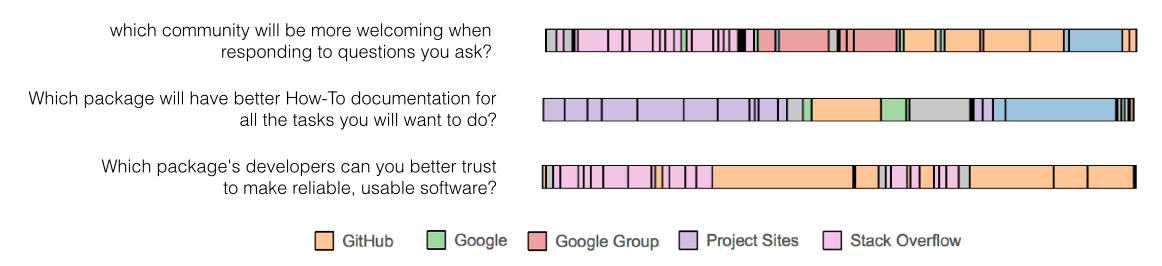
\includegraphics[width=0.9\textwidth]{figures/visits}
\caption{%
The sequence of communication channels one developer visited when answering questions that ask them to compare the quality of packages' community, documentation, and developers.
Though we have found that users often rely on different channels, though this one relies on an interesting assortment:
project documentation, GitHub, and blog posts to learn about the availale How-To documentation;
Stack Overflow, Reddit, and Google Groups to learn about how welcoming the community is;
GitHub profile pages, issues, pull request, and Stack Overflow to learn more about the developers behind the package.
}
\label{fig:visits}
\end{figure*}

There are several online tools we see as precursors to much more powerful socially-enabled telemetry systems.
%Slant\footnote{\url{http://www.slant.co/}} allows developers to request comparisons of alternatives of packages for programming tasks like drawing libraries and package managers through bite-sized bullet point pros and cons written by peers.
Awesome Python\footnote{\url{https://python.libhunt.com/}} generates comparisons of arbitrary pairs of Python packages\footnote{\url{https://python.libhunt.com/project/pygame/vs/panda3}}, with popularity and activity metrics presumably based on download counts and commit activity.
Ruby Toolbox\footnote{\url{https://www.ruby-toolbox.com/}} and the `packagequality' widget\footnote{\url{http://packagequality.com/}} compute package quality ratings that draw on download counts, responses to issues, and GitHub stars.
While these can be proxies for a package's quality, we believe that this isn't enough for understanding the social life of packages.
When using packages, developers are concerned with the trustworthiness of developers~\cite{robillard_field_2011}, how up-to-date the documentation is~\cite{storey_revolution_2014,nykaza_what_2002,lethbridge_how_2003,robillard_field_2011}, and whether the community is anti-social~\cite{storey_revolution_2014}.

As developers will often have to make trade-offs between these factors when choosing software, we are skeptical that anything short of carefully selected and arranged samples from socially-enabled channels can help a developer make a truly informed judgment about a package's community when evaluating software and, after on-boarding, choosing how to ask for help.
This abstract presents our inquiry into what these samples from developers' socially-enabled networks and web pages should be.

\if 0
Software developers decide to reuse software to save time~\cite{mili_reusing_1995}.
Researchers have observed that given a task, developers can assemble working programs through components found entirely on the web, together with their prior knowledge (e.g.,~\cite{brandt_two_2009}).
This behavior is not uncommon---foraging for information online has been observed in particular for a variety of non-professional programmers~\cite{brandt_opportunistic_2008} and validated through the queries for a help search engine for developer tools~\cite{brandt_two_2009}.

Though there are hazards in how developers select reusable components for software in practice.
A premium is placed on working source code examples~\cite{nykaza_what_2002}.
Developers' tend to choose code that ``satisfices'' without thoroughly testing it~\cite{brandt_two_2009}.
APIs have unexpected and undocumented side effects~\cite{robillard_field_2011}.
And despite a rise of ``socially enabled'' digital media for communicating about software, programmers face challenges using these channels:
they may be overwhelmed by the amount of content and distrust its quality~\cite{storey_revolution_2014}.

In this study, we present a view of how developers learn about packages on socially enabled channels.
Through this study, we highlight two problems:
First, programmers attempt to make sense of distributed information online.
Second, some information is hidden from view, only to be discovered after tens of minutes of inspection.
For us, these findings will motivate the design of new search systems for developers looking for resuable software components.
\fi

% We believe that such representations, shown in the right place when developers are choosing new components, reduce the hazards of poor reuse choices when developers lack media literacy, and can help programmers understand what components are safe to trust.

\if 0
The past five decades of software engineering have seen the rise of digital media for programmer communication and information sharing.
As of the '90s, the web has ``socially enabled'' many new digital media, transforming how developers learn about new technologies~\cite{storey_revolution_2014}.
In the last ten years, millions of projects migrated to GitHub, a social code hosting site, and hundreds of thousands of packages of reusable software have been published on globally available and instantly accessible ``package indexes'' for the Ruby, JavaScript, and Python languages.
Not only has reusable software moved online en masse, but so too has much of the documentation for this work.

In this paper, we describe how indications of content quality can be harvested on a package level from four top digital channels that developers use for development~\cite{storey_revolution_2014}, three of which are socially enabled: code hosting, Q\&A sites, web search, and micro-blogging.
We focus specifically on reusable components at the resolution of packages, or self-contained libraries that can be installed from a package index and easily imported into one's code.
We make this choice as packages have a system image that, although distributed and ``fragmented,'' is accessible through thoughtful and systematized queries to the search interfaces and APIs of social media and web search.

Our primary contribution is that we build a system that creates summaries of package support quality by collecting fragmented information across digital channels and summarizes them in lightweight representations.
We report how developers perceive the trustworthiness of software given these representations.
We then suggest which channels appear to be the richest for conveying variation on the quality of reusable components to developers who have not seen them before.
We present several example interfaces that show how these indications can be incorporated into modern interfaces where programmers seek help and may encounter the option to install packages.
\fi


% \section{Background}
% Developers work in an immense online network.
Developers benefit from this network by
leveraging social media and other channels to stay informed
and connect with other developers~\cite{singer_software_2014,storey_how_2016}.
Today there is a proliferation of socially-enabled channels~\cite{storey_revolution_2014} through which developers
answer each other's questions~\cite{mamykina_fastest_2011},
stay up-to-speed with rapidly changing software~\cite{linares-vasquez_how_2014},
help each other overcome bugs and learn new tools~\cite{parnin_blogging_2013},
and share information in many different forms at many different speeds.
The knowledge and conversations of programmers are increasingly distributed across the web.

Some community-developed tools aim to help developers compare packages.
Such community tools only show a fraction of the metrics used by developers.
Typical metrics for these tools (e.g.,~\cite{awesome_python,package_quality,ruby_toolbox}) tend to be based on counts and rates of code contributions, issue resolutions, downloads, and ``stars'' on code hosting sites like GitHub.
% Awesome Python\footnote{\url{https://python.libhunt.com/}} generates comparisons of arbitrary pairs of Python packages\footnote{\url{https://python.libhunt.com/project/pygame/vs/panda3}}, with an activity metrics based on commit frequency and an opaque numerical measurement of popularity.
% uby Toolbox\footnote{\url{https://www.ruby-toolbox.com/}} and the `packagequality' widget\footnote{\url{http://packagequality.com/}} also summarize package qualities with numerical ratings, where `packagequality' relies on issue response rates, download count, and version count.
% This isn't enough.
Developers may be concerned with
how much they respect the authors of code~\cite{robillard_field_2011},
how up-to-date the documentation is~\cite{lethbridge_how_2003,nykaza_what_2002,robillard_field_2011,storey_revolution_2014},
and whether the community is anti-social~\cite{storey_revolution_2014}.
We propose that carefully selected samples from communication channels can help developers make more informed judgments based on social health.
The current work presents a study to help us pick these samples.
% Developers will often have to make trade-offs between these factors when choosing software.
% In this abstract, we ask what these samples from developers' socially-enabled networks and web pages should be.

\if 0

Storey et al.~\cite{storey_revolution_2014}, in their survey of developers' use of media channels, present a list of digital channels, and digital channels enabled with social media, that we find to be representative of the channels that developers use for support.
In their survey, Storey et al.\ ask developers to name three channels that they find most important for development.
In our analysis, we focus on some of the top digital channels that developers mentioned the most, including code hosting, Q\&A, web search, and micro-blogging.
% We do not report non-digital channels, as from our review, these don't seem to have the same hazards of fragmented or missing information and anti-social behavior that was reported as being problematic for digital channels.

% The first three of these were explicitly mentioned in the three interviews we conducted with participants.
% We feel concentrating on these channels provides a diversity of channels, with different ways of communicating and finding information.

Developers face challenges when seeking support for software that they are reusing.
The right information is often missing in the place that developers are looking for it~\cite{robillard_field_2011,storey_revolution_2014,nykaza_what_2002}.
The right components may be accessible only with terms or concepts the developer isn't familiar with~\cite{nykaza_what_2002,jeong_improving_2009,robillard_field_2011} or require dependencies the developer doesn't know how to use.
Developers can find documentation untrustworthy~\cite{robillard_field_2011,storey_revolution_2014}, misleading, wrong, and out of date~\cite{nykaza_what_2002,lethbridge_how_2003,robillard_field_2011}.
The speed of answers on mailing lists and Q\&A sites can vary and take longer than developers want; slow response times can deter developers from asking questions or using a library.
Furthermore, information can be organized in a way that developers find costly to navigate~\cite{robillard_field_2011}, and can be fragmented in a way that requires developers to look in multiple places to find the information they need~\cite{jeong_improving_2009}.

There are already signals that programmers use to determine choices about trusting information and how to seek support online.
Some developers may rely on experience and intuition~\cite{storey_revolution_2014}.
They may inspect cosmetic features of web pages~\cite{brandt_two_2009}.
Authority and credibility of code examples can be assessed based on knowledge of and respect for the author of the code and evidence that the example is up to date~\cite{robillard_field_2011}.
% One of our interview participants mentioned that they are more likely to write bug reports to project authors that have a history or responsiveness (P2).
In short, there is evidence that surface-level features help in the moment when deciding whether to make use of online documents, and an understanding of project authors' background and history can help a developer decide what components to use and when to ask questions.

\fi

\if 0
During exploratory literature reviews, we encountered research in computer-supported cooperative work that offered interfaces to help readers assess the quality of socially curated content.
Examples of representations include: heat maps of readers' judgments of article credibility~\cite{pirolli_so_2009};
vignettes and text formatting revealing discussion and conflict around content snippets~\cite{towne_your_2013,borra_societal_2015};
visualizations of wiki contributions by user~\cite{arazy_recognizing_2010};
change request activity during development~\cite{begel_codebook_2010};
and groups of open source project commit messages, clustered by topic~\cite{hindle_whats_2009}.
From this small and very non-random sample, we have anecdotal evidence that there is research interest in providing front ends to help consumers of social content share opinions about credibility, assess authorship, and to coordinate teamwork.
\fi

\if 0
Programming is an incredibly information intensive activity.
What's more, for many programmers and software development activities, information seeking and code reuse is inseparable from programming.
As an example, consider the study by Brandt et al.~\cite{brandt_two_2009}.

Our work is motivated by an observation from a previous thread of research.
When interviewing a developer of programming documentation, we began to talk about ``badges.''
Badges are small indicators packaged in a standardized form that convey some single scalar dimension of the quality of the project:
for example, whether there is a chat channel for it, the number of stars on GitHub, and the percentage of code exercised by unit tests.

From personal experience, we knew that the story of finding support for a package is complex, rich, and immensely varied, even for a single package.
It would be comical to try to distill a sense of the entirety of support, strewn out over the web, into a very small space.
But we recognized that due to the developing norms of increasingly active online open source community, and the standard methods of access for this information (that is, using Google), fetching and interpreting a wide coverage of information for packages systematically is not out of the question.
So this is what we sought out to do.

This paper makes a mixed-methods contribution.
The primary enabler of this contribution is a system that, on-demand, captures longitudinal indicators of support that includes official documentation, Q\&A, and perhaps most uniquely, tutorial content.
To convey the complexity of finding packages with the right support, we conduct a handful of interviews with programmers from various backgrounds, revealing strategies, concerns, and pitfalls of working with online support for a package over a long lifetime of reuse.
To show that this data can be used in meaningful user-facing representations, we design a search user interface with the story of intending to help programmers select the right packages.
An evaluation in the lab shows that such representations, based on already-available (but currently distributed) data has the potential to change how programmers seek reusable programming components.
We leave the problem of wrapping this data for software developers as a method for ``software support telemetry'' as an item of future work for ourselves.

We believe that our techniques are applicable to creating user-facing indicators of online support for communities besides programmers.
This includes\ldots{}.
\fi


\section{Our Approach}
% To answer this question, we present preliminary results from an in-progress study.
We invited 10 developers to a study where they compared the social health of two packages.
Each participant chose a pair of packages, out of three pairs.
% Each pair was for a different programming task.
Then we asked the participant to compare the two packages, using six questions about each package's community, documentation, and developers.
The questions were based on related work and conversations we had with software developers, and included:
\begin{itemize}
\setlength{\itemsep}{0pt}
\setlength{\parskip}{0pt}
\setlength{\parsep}{0pt}  
\item Which community will be more welcoming when responding to questions you ask?
\item Which package's documentation will be more up-to-date with the code?
\item Which package's developers can you better trust to make reliable, usable software?
\end{itemize}
These three questions (out of six) were based on observations of anti-social behavior in developers' communication channels~\cite{storey_revolution_2014}, concerns about how up-to-date documentation is~\cite{storey_revolution_2014,nykaza_what_2002,lethbridge_how_2003,robillard_field_2011}, and how developers assess code example quality based on author reputation~\cite{robillard_field_2011}.
% These questions were chosen based on related work (including~\cite{storey_revolution_2014,nykaza_what_2002,lethbridge_how_2003,robillard_field_2011}) and conversations with software developers.

Participants answered the questions using the web.
We note developers often get answers face-to-face~\cite{latoza_maintaining_2006,storey_revolution_2014}, over email~\cite{latoza_maintaining_2006,ko_information_2007}, or by trying out code~\cite{brandt_two_2009}.
However, we focused on information on the web, as we believed this would reveal signals we could incorporate into future search tools.

We collected three measurements of cues participants used to answer social questions:
a timestamped log of visited URLs;
self-reported ratings of web pages' ``helpfulness'' for answering each question;
and open-ended responses of what evidence on the web was most helpful for comparing the social health of the two packages for each question.
We report a view of our current results here.
Our on-going analysis has focused on two research questions:
(1) What sites do participants use to learn about a package's social health?
(2) What challenges do developers face when learning about a package's social health?

\if 0

The objective for this study is to answer these questions.
First, what channels are most helpful to developers predicting the quality of community and documentation available for packages?
Second, what information and indications do they use from these channels to answer these questions?
Third, what challenges do developers face when answering each question?

We designed a study to elicit answers to these questions.
Participants were given the names of two Python packages that they were supposed to compare in terms of quality of community and documentation.
These packages were chosen related to a task the participant expressed interest in, though we made sure the participant had never used either of the packages before.

We asked developers to attempt to answer six questions about the quality of the community and documentation:
\begin{enumerate}
\setlength{\itemsep}{0pt}
\setlength{\parskip}{0pt}
\setlength{\parsep}{0pt}
\item Which package's \textbf{developers can you better trust} to make reliable, usable software?
\item Which community will be more \textbf{welcoming} when responding to questions you ask?
\item Which package will have \textbf{better How-To documentation} for all the tasks you will want to do?
\item Which package was better designed for users with \textbf{your technical knowledge} and goals?
\item For which package are other developers more likely to answer questions you ask as \textbf{fast} as you need them to?
\item Which package's documentation will be more \textbf{up-to-date} with the code?
\end{enumerate}
These questions came from a variety of sources referenced in our background work and from our peers.
We had a hunch that there might be some appropriate information sources online for answering each of these questions, but we didn't know for sure, or the variety of different approaches that developers might take.
For each question, participants were given six minutes to use the web to learn more about the two packages they were comparing, in order to arrive at an informed answer.
\textbf{Warmup task}.

We collected a variety of measures.
We logged all URLs that participants visited along with timestamps of how long they spent on each site to determine how much time they were spending on each site to answer each question.
We also requested that participants report the helpfulness of pages that they visited as ``very helpful'', ``somewhat helpful'', or ``not helpful'' for answering each question.
(In practice, we had to remind them of this quite frequently, and received sparse ratings that did not cover many of the pages visited).
We also asked participants to report their confidence in their comparison between the two packages, knowing that participants may only find a fraction of the available information on the web and in the time frame we gave them.

We also asked participants to produce two forms of written feedback.
Before they began to search to answer this question, they were asked to share a 1--2 sentence strategy of how they expected to find an answer to the question.
We expect this not only allowed participants to mentally prepare for the upcoming task, but also allowed us to ask after the study which of their strategies didn't succeed.
After they searched, we asked them to report what evidence they found most helpful for comparing the two packages.

We have currently run the study with ten participants.
\textbf{These participants have this background\ldots{}}.
We report the results in the next section.

We have made our Firefox addon for logging URL activity open source and available to the research community\footnote{\url{https://github.com/andrewhead/Web-Navigation-Logger}}.

% These questions are pretty vague.
% We think this is okay, because the task of assessing the documentation and support for a package is going to involve some prediction of the types of information needs one will need later, and is fundamentally a difficult and ill-posed problem.

\fi

\if 0
\subsection{Procedure}

A participant is provided a web domain for a digital channel (GitHub, Stack Overflow, or Google search), and is asked to spend time on that domain (and that domain only) assessing the project's quality on one of the questions of quality.
They do this $3\times3$ times, for 3 channels and 3 questions of quality.

This design is within-subjects: all participants answer all questions for all channels.
This provides us with additional information per participant.
It also allows us to make claims based on how ratings for each question-channel pair vary between participants.
We counterbalance the order of channels and questions to reduce the effect of learning on task completion, certainty, and ratings of quality.
We use a separate Node package for each task.

Each trial lasted at maximum 3 minutes long.
Though participants could finish early if they felt they found all relevant information.
After this time, participants were asked to stop and save their rating of quality and any notes they share.
Participants were asked for their feedback in a Google Form.

% In the current design, participants will be given three minutes for each task, but can finish as quickly as they want.
% There will be three channels (code hosting site, Q\&A site, and micro-blogging site) and three questions (see the questions in the ``motivation'' section).
We were originally planning on testing out a micro-blogging site, but during test runs with themselves, the researchers discovered that there these questions were difficult enough to answer with Twitter that it would be more interesting to see what participants did with Google search.
With one minute between tasks, the main activity was expected to take 40--50 minutes total.

We collected information about participants' demographics and background in a preliminary questionnaire.
Participants performed a three-minute warmup task to familiarize themselves with the form and adjust to the time constraints we provided.
Participants then completed a follow-up questionnaire where they were asked to rank channels by their effectiveness in answering each of the questions, describe what they found to be the most helpful cues overall for each question, and mention other sources of information they would want to see.
\fi

\if 0
There is a covariate with the combination of channel and question: the package itself.
If we do not include this covariate, there will be a learning confound from participants gaining knowledge about the support available for the package from past trials.
We don't counterbalance the order of packages.
We think this is okay, because we are not comparing for which packages quality is easiest to assess.
We're only comparing which sites and questions are easier to answer questions about, and each site and question will get an equal distribution of each of the packages.
Furthermore, the counterbalancing starts to get unintuitive and hard to follow at this point.

We show some helpful notes for some of the packages.
For instance, we explain that the ``python'' package is a package for Node.js, and not the Python language.
We think that this is okay because we don't let participants view Google and so might need to give them some cues to make information discovery for the package tractable.
Furthermore, we don't worry about biasing the results for individual packages for the reasons in the paragraph above.
\fi

\if 0
To obtain a list of packages, I suggest fetching packages that participants are not certain to know (i.e.\ ones that aren't ubiquitous within the Node.js ecosystem), and that represent varying levels of popularity online.
We make a heuristic for packages that have some documentation online.
We look for the pattern \texttt{npm install <package\_name>} in all Stack Overflow posts tagged ``node.js'' or ``npm,'' and extract all distinct package names, counting how often that package name appears.
We choose three packages from each of these percentile ranges: 5--10\%, 10--30\%, 30--100\%.
We note that this might confound the Stack Overflow condition, as all packages will have at least a trivial amount of documentation.

Some participants may already know about some of the packages and authors that we show them, if they have some level of community support and the developer has been working with Node.js for some time.
We ask all participants to check boxes to report whether they have heard of and whether they have used each package.
 We can use this to exclude some ratings from our analysis.
 If they know of authors, this might not be problematic, as this could be indicative of a need to summarize packages in terms of those who created them.
\fi
\if 0
\subsection{Measures}

\begin{itemize}
\item their confidence in their judgment
\item whether a participant completes a task in less time than was available 
\item ratings on a Likert scale of each quality question
\end{itemize}

There are auxiliary questions that it would be useful for us to report on:
* How confident are participants of their responses?
* How does this confidence vary by channel and question?
* How appropriate does this channel's content and organization seem for answering this question?
* For each package, how often to participants end up looking at documentation that's not about that package at all (by accident)?

\subsection{Analysis}

We use the technique described in~\cite{kaptein_powerful_2010} to assess whether there is a difference between the distributions of confidence scores for both factors.
According to the recommendations from\footnote{\url{http://yatani.jp/teaching/doku.php?id=hcistats:kruskalwallis}}, we use a Mann-Whitney test for post-hoc pairwise comparisons.
In this way, we report which channels appear to be most capable of answering each question.

Confidence scores will also be useful in initially assessing whether there is any distribution for which confidence is more than positive.
If this assumption holds, then we can assert that there indeed are some channels for which such quality assessments are possible.

We do a qualitative coding of participants' comments for evidence of the cues and challenges of using each channel to answer these question; we will not look for quantitative significance in comments.

\subsection{Limitations}

We report some biases in the study design.
One of the reasons that we include web search is because we already have some code written to collect data about web search, and an on-going theme of our work is to understand how to help programmers search better.

The script that we used to generate forms for our study can be found online at \url{http://tinyurl.com/support-views-study-script}.
\fi


\section{Preliminary Results}
We observed several noteworthy strategies participants took to learn about a package's social health.
First, participants read relevant text to assess social health.
In particular, participants skimmed text from conversations to determine how welcoming communities were.
Participants also read texts from documentation about a project's API and development philosophy to determine if a package was designed for users with their backgrounds and goals.
Existing package comparison tools do not support reading relevant conversations and documentation.
Instead, such tools only show summary statistics (e.g.~\cite{awesome_python,ruby_toolbox}).

Participants sometimes looked for social health cues in the form of advice from current users of a package.
Participants queried the web through search engines to find pre-built summaries describing the community and documentation.
Participants found explicit comparisons of packages on Reddit, and user testimonials on Quora.
One participant consulted issue reports to determine how up-to-date documentation was.
% On these channels, the presence or absence of information can be an answer in itself.
When participants looked at texts of questions, documents, and issue reports, they chose a handful of pages from dozens or even hundreds.
% While their choices appeared to be informed at least partly by what appeared on the pages they were currently visiting, we hope future analysis will provide further insight into just how participants chose pages to visit.

% We are in the process of collecting developers' pathways through web documents when they answer social questions about packages.
Our URL log data suggests common places where participants found social health cues.
Participants relied on different types of web pages when answering each social health question.
% Developers visited important communication channels~\cite{storey_revolution_2014}, including code hosting, web search, and Q\&A sites.
We have seen participants find:
(1) whether a community is welcoming by viewing Q\&A sites and discussions on Reddit and Google Groups;
(2) documentation recency by viewing issue reports, code contribution histories, and pull request contents;
(3) the trustworthiness of developers by viewing issue reports, and profiles on code hosting sites.
Figure~\ref{fig:visits} shows a cross-section of the URLs one participant visited when answering three of the six questions.
We leave quantitative analysis of these trends and a full exploration of specific cues from these sites for future work.

Our preliminary results confirm a need for search tools that reveal obscure information about social health quickly.
Participants frequently realized they missed important information after twenty or thirty minutes of learning about a package.
One participant wrongly assessed a package had no community at all.
Another participant failed to find newer version of a package under a different name.
And another participant missed large repositories of example code written by the package's developers.
%searching that changes their perception of a package, often only after the right question is asked---for example, discovering that a package's primary maintainer has been inactive for two years.
Such incorrect judgments could be costly to reverse:
One participant read source code before realizing that one package's programming API was preferable to one he favored before.

We believe these incorrect judgments are a product of developers' habits and the limitations of current information interfaces.
With attention to both, we can design more powerful search tools to help developers quickly and effectively learn about packages' social health when choosing between them.
For now, these preliminary results suggest that
package consumers should not trust their initial instincts,
and should inspect comparisons, discussions, and Q\&A for a well-informed picture of a package's social health.
Developers should know that cues about the social health for their projects could exist on dozens of domains,
and potential consumers may need help learning where to look for help.

\if 0
Include the major insights that developers had during the study.
For example:
there's a new major version;
there's an examples repository that wasn't clearly shown;
there's a Google Groups page for the project;
the docs are actually pretty usable.
From this (and hopefully other insights) we see that a surface appearance of a package takes a while to build up accurately, and might require looking at a package from multiple different angles.
We think that it need not take so much time.

Not all developers seemed to agree on what information sources were best.
Part of this is likely because of prior knowledge.
One of the participants chose to look at the IRC channels for the package.

I want to touch upon each of the following.

What questions are participants least confident answering?

What are the most authoratative sources for answering each question?

What do they approximate to aggregate?

How much do participants' perceptions of documentation change?  And how much do their opinions change?

And what does this all suggest for what's broken for information presentation, and the design of programmers' front-end to the web?
\fi


\if 0
The \textit{proceedings} are the records of a conference.
ACM seeks to give these conference by-products a uniform,
high-quality appearance.  To do this, ACM has some rigid
requirements for the format of the proceedings documents: there
is a specified format (balanced  double columns), a specified
set of fonts (Arial or Helvetica and Times Roman) in
certain specified sizes (for instance, 9 point for body copy),
a specified live area (18 $\times$ 23.5 cm [7" $\times$ 9.25"]) centered on
the page, specified size of margins (1.9 cm [0.75"]) top, (2.54 cm [1"]) bottom
and (1.9 cm [.75"]) left and right; specified column width
(8.45 cm [3.33"]) and gutter size (.83 cm [.33"]).

The good news is, with only a handful of manual
settings\footnote{Two of these, the {\texttt{\char'134 numberofauthors}}
and {\texttt{\char'134 alignauthor}} commands, you have
already used; another, {\texttt{\char'134 balancecolumns}}, will
be used in your very last run of \LaTeX\ to ensure
balanced column heights on the last page.}, the \LaTeX\ document
class file handles all of this for you.

The remainder of this document is concerned with showing, in
the context of an ``actual'' document, the \LaTeX\ commands
specifically available for denoting the structure of a
proceedings paper, rather than with giving rigorous descriptions
or explanations of such commands.

\section{The {\secit Body} of The Paper}
Typically, the body of a paper is organized
into a hierarchical structure, with numbered or unnumbered
headings for sections, subsections, sub-subsections, and even
smaller sections.  The command \texttt{{\char'134}section} that
precedes this paragraph is part of such a
hierarchy.\footnote{This is the second footnote.  It
starts a series of three footnotes that add nothing
informational, but just give an idea of how footnotes work
and look. It is a wordy one, just so you see
how a longish one plays out.} \LaTeX\ handles the numbering
and placement of these headings for you, when you use
the appropriate heading commands around the titles
of the headings.  If you want a sub-subsection or
smaller part to be unnumbered in your output, simply append an
asterisk to the command name.  Examples of both
numbered and unnumbered headings will appear throughout the
balance of this sample document.

Because the entire article is contained in
the \textbf{document} environment, you can indicate the
start of a new paragraph with a blank line in your
input file; that is why this sentence forms a separate paragraph.

\subsection{Type Changes and {\subsecit Special} Characters}
We have already seen several typeface changes in this sample.  You
can indicate italicized words or phrases in your text with
the command \texttt{{\char'134}textit}; emboldening with the
command \texttt{{\char'134}textbf}
and typewriter-style (for instance, for computer code) with
\texttt{{\char'134}texttt}.  But remember, you do not
have to indicate typestyle changes when such changes are
part of the \textit{structural} elements of your
article; for instance, the heading of this subsection will
be in a sans serif\footnote{A third footnote, here.
Let's make this a rather short one to
see how it looks.} typeface, but that is handled by the
document class file. Take care with the use
of\footnote{A fourth, and last, footnote.}
the curly braces in typeface changes; they mark
the beginning and end of
the text that is to be in the different typeface.

You can use whatever symbols, accented characters, or
non-English characters you need anywhere in your document;
you can find a complete list of what is
available in the \textit{\LaTeX\
User's Guide}\cite{Lamport:LaTeX}.

\subsection{Math Equations}
You may want to display math equations in three distinct styles:
inline, numbered or non-numbered display.  Each of
the three are discussed in the next sections.

\subsubsection{Inline (In-text) Equations}
A formula that appears in the running text is called an
inline or in-text formula.  It is produced by the
\textbf{math} environment, which can be
invoked with the usual \texttt{{\char'134}begin. . .{\char'134}end}
construction or with the short form \texttt{\$. . .\$}. You
can use any of the symbols and structures,
from $\alpha$ to $\omega$, available in
\LaTeX\cite{Lamport:LaTeX}; this section will simply show a
few examples of in-text equations in context. Notice how
this equation: \begin{math}\lim_{n\rightarrow \infty}x=0\end{math},
set here in in-line math style, looks slightly different when
set in display style.  (See next section).

\subsubsection{Display Equations}
A numbered display equation -- one set off by vertical space
from the text and centered horizontally -- is produced
by the \textbf{equation} environment. An unnumbered display
equation is produced by the \textbf{displaymath} environment.

Again, in either environment, you can use any of the symbols
and structures available in \LaTeX; this section will just
give a couple of examples of display equations in context.
First, consider the equation, shown as an inline equation above:
\begin{equation}\lim_{n\rightarrow \infty}x=0\end{equation}
Notice how it is formatted somewhat differently in
the \textbf{displaymath}
environment.  Now, we'll enter an unnumbered equation:
\begin{displaymath}\sum_{i=0}^{\infty} x + 1\end{displaymath}
and follow it with another numbered equation:
\begin{equation}\sum_{i=0}^{\infty}x_i=\int_{0}^{\pi+2} f\end{equation}
just to demonstrate \LaTeX's able handling of numbering.

\subsection{Citations}
Citations to articles \cite{bowman:reasoning,
clark:pct, braams:babel, herlihy:methodology},
conference proceedings \cite{clark:pct} or
books \cite{salas:calculus, Lamport:LaTeX} listed
in the Bibliography section of your
article will occur throughout the text of your article.
You should use BibTeX to automatically produce this bibliography;
you simply need to insert one of several citation commands with
a key of the item cited in the proper location in
the \texttt{.tex} file \cite{Lamport:LaTeX}.
The key is a short reference you invent to uniquely
identify each work; in this sample document, the key is
the first author's surname and a
word from the title.  This identifying key is included
with each item in the \texttt{.bib} file for your article.

The details of the construction of the \texttt{.bib} file
are beyond the scope of this sample document, but more
information can be found in the \textit{Author's Guide},
and exhaustive details in the \textit{\LaTeX\ User's
Guide}\cite{Lamport:LaTeX}.

This article shows only the plainest form
of the citation command, using \texttt{{\char'134}cite}.
This is what is stipulated in the SIGS style specifications.
No other citation format is endorsed or supported.

\subsection{Tables}
Because tables cannot be split across pages, the best
placement for them is typically the top of the page
nearest their initial cite.  To
ensure this proper ``floating'' placement of tables, use the
environment \textbf{table} to enclose the table's contents and
the table caption.  The contents of the table itself must go
in the \textbf{tabular} environment, to
be aligned properly in rows and columns, with the desired
horizontal and vertical rules.  Again, detailed instructions
on \textbf{tabular} material
is found in the \textit{\LaTeX\ User's Guide}.

Immediately following this sentence is the point at which
Table 1 is included in the input file; compare the
placement of the table here with the table in the printed
dvi output of this document.

\begin{table}
\centering
\caption{Frequency of Special Characters}
\begin{tabular}{|c|c|l|} \hline
Non-English or Math&Frequency&Comments\\ \hline
\O & 1 in 1,000& For Swedish names\\ \hline
$\pi$ & 1 in 5& Common in math\\ \hline
\$ & 4 in 5 & Used in business\\ \hline
$\Psi^2_1$ & 1 in 40,000& Unexplained usage\\
\hline\end{tabular}
\end{table}

To set a wider table, which takes up the whole width of
the page's live area, use the environment
\textbf{table*} to enclose the table's contents and
the table caption.  As with a single-column table, this wide
table will ``float" to a location deemed more desirable.
Immediately following this sentence is the point at which
Table 2 is included in the input file; again, it is
instructive to compare the placement of the
table here with the table in the printed dvi
output of this document.


\begin{table*}
\centering
\caption{Some Typical Commands}
\begin{tabular}{|c|c|l|} \hline
Command&A Number&Comments\\ \hline
\texttt{{\char'134}alignauthor} & 100& Author alignment\\ \hline
\texttt{{\char'134}numberofauthors}& 200& Author enumeration\\ \hline
\texttt{{\char'134}table}& 300 & For tables\\ \hline
\texttt{{\char'134}table*}& 400& For wider tables\\ \hline\end{tabular}
\end{table*}
% end the environment with {table*}, NOTE not {table}!

\subsection{Figures}
Like tables, figures cannot be split across pages; the
best placement for them
is typically the top or the bottom of the page nearest
their initial cite.  To ensure this proper ``floating'' placement
of figures, use the environment
\textbf{figure} to enclose the figure and its caption.

This sample document contains examples of \textbf{.eps} files to be
displayable with \LaTeX.  If you work with pdf\LaTeX, use files in the
\textbf{.pdf} format.  Note that most modern \TeX\ system will convert
\textbf{.eps} to \textbf{.pdf} for you on the fly.  More details on
each of these is found in the \textit{Author's Guide}.

\begin{figure}
\centering
\includegraphics{fly}
\caption{A sample black and white graphic.}
\end{figure}

\begin{figure}
\centering
\includegraphics[height=1in, width=1in]{fly}
\caption{A sample black and white graphic
that has been resized with the \texttt{includegraphics} command.}
\end{figure}


As was the case with tables, you may want a figure
that spans two columns.  To do this, and still to
ensure proper ``floating'' placement of tables, use the environment
\textbf{figure*} to enclose the figure and its caption.
and don't forget to end the environment with
{figure*}, not {figure}!

\begin{figure*}
\centering
\includegraphics{flies}
\caption{A sample black and white graphic
that needs to span two columns of text.}
\end{figure*}


\begin{figure}
\centering
\includegraphics[height=1in, width=1in]{rosette}
\caption{A sample black and white graphic that has
been resized with the \texttt{includegraphics} command.}
\vskip -6pt
\end{figure}

\subsection{Theorem-like Constructs}
Other common constructs that may occur in your article are
the forms for logical constructs like theorems, axioms,
corollaries and proofs.  There are
two forms, one produced by the
command \texttt{{\char'134}newtheorem} and the
other by the command \texttt{{\char'134}newdef}; perhaps
the clearest and easiest way to distinguish them is
to compare the two in the output of this sample document:

This uses the \textbf{theorem} environment, created by
the\linebreak\texttt{{\char'134}newtheorem} command:
\newtheorem{theorem}{Theorem}
\begin{theorem}
Let $f$ be continuous on $[a,b]$.  If $G$ is
an antiderivative for $f$ on $[a,b]$, then
\begin{displaymath}\int^b_af(t)dt = G(b) - G(a).\end{displaymath}
\end{theorem}

The other uses the \textbf{definition} environment, created
by the \texttt{{\char'134}newdef} command:
\newdef{definition}{Definition}
\begin{definition}
If $z$ is irrational, then by $e^z$ we mean the
unique number which has
logarithm $z$: \begin{displaymath}{\log e^z = z}\end{displaymath}
\end{definition}

Two lists of constructs that use one of these
forms is given in the
\textit{Author's  Guidelines}.
 
There is one other similar construct environment, which is
already set up
for you; i.e. you must \textit{not} use
a \texttt{{\char'134}newdef} command to
create it: the \textbf{proof} environment.  Here
is a example of its use:
\begin{proof}
Suppose on the contrary there exists a real number $L$ such that
\begin{displaymath}
\lim_{x\rightarrow\infty} \frac{f(x)}{g(x)} = L.
\end{displaymath}
Then
\begin{displaymath}
l=\lim_{x\rightarrow c} f(x)
= \lim_{x\rightarrow c}
\left[ g{x} \cdot \frac{f(x)}{g(x)} \right ]
= \lim_{x\rightarrow c} g(x) \cdot \lim_{x\rightarrow c}
\frac{f(x)}{g(x)} = 0\cdot L = 0,
\end{displaymath}
which contradicts our assumption that $l\neq 0$.
\end{proof}

Complete rules about using these environments and using the
two different creation commands are in the
\textit{Author's Guide}; please consult it for more
detailed instructions.  If you need to use another construct,
not listed therein, which you want to have the same
formatting as the Theorem
or the Definition\cite{salas:calculus} shown above,
use the \texttt{{\char'134}newtheorem} or the
\texttt{{\char'134}newdef} command,
respectively, to create it.

\subsection*{A {\secit Caveat} for the \TeX\ Expert}
Because you have just been given permission to
use the \texttt{{\char'134}newdef} command to create a
new form, you might think you can
use \TeX's \texttt{{\char'134}def} to create a
new command: \textit{Please refrain from doing this!}
Remember that your \LaTeX\ source code is primarily intended
to create camera-ready copy, but may be converted
to other forms -- e.g. HTML. If you inadvertently omit
some or all of the \texttt{{\char'134}def}s recompilation will
be, to say the least, problematic.
\fi

\section{Conclusions}
In summary, we rock.

\if 0
This paragraph will end the body of this sample document.
Remember that you might still have Acknowledgments or
Appendices; brief samples of these
follow.  There is still the Bibliography to deal with; and
we will make a disclaimer about that here: with the exception
of the reference to the \LaTeX\ book, the citations in
this paper are to articles which have nothing to
do with the present subject and are used as
examples only.
\fi
%\end{document}  % This is where a 'short' article might terminate

%ACKNOWLEDGMENTS are optional
\if 0
\section{Acknowledgments}
This section is optional; it is a location for you
to acknowledge grants, funding, editing assistance and
what have you.  In the present case, for example, the
authors would like to thank Gerald Murray of ACM for
his help in codifying this \textit{Author's Guide}
and the \textbf{.cls} and \textbf{.tex} files that it describes.
\fi

%
% The following two commands are all you need in the
% initial runs of your .tex file to
% produce the bibliography for the citations in your paper.
\bibliographystyle{abbrv}
\bibliography{sigproc}  % sigproc.bib is the name of the Bibliography in this case
% You must have a proper ".bib" file
%  and remember to run:
% latex bibtex latex latex
% to resolve all references
%
% ACM needs 'a single self-contained file'!
%
%APPENDICES are optional
%\balancecolumns
\if 0 
\appendix
%Appendix A
\section{Headings in Appendices}
The rules about hierarchical headings discussed above for
the body of the article are different in the appendices.
In the \textbf{appendix} environment, the command
\textbf{section} is used to
indicate the start of each Appendix, with alphabetic order
designation (i.e. the first is A, the second B, etc.) and
a title (if you include one).  So, if you need
hierarchical structure
\textit{within} an Appendix, start with \textbf{subsection} as the
highest level. Here is an outline of the body of this
document in Appendix-appropriate form:
\subsection{Introduction}
\subsection{The Body of the Paper}
\subsubsection{Type Changes and  Special Characters}
\subsubsection{Math Equations}
\paragraph{Inline (In-text) Equations}
\paragraph{Display Equations}
\subsubsection{Citations}
\subsubsection{Tables}
\subsubsection{Figures}
\subsubsection{Theorem-like Constructs}
\subsubsection*{A Caveat for the \TeX\ Expert}
\subsection{Conclusions}
\subsection{Acknowledgments}
\subsection{Additional Authors}
This section is inserted by \LaTeX; you do not insert it.
You just add the names and information in the
\texttt{{\char'134}additionalauthors} command at the start
of the document.
\fi
\if 0
\subsection{References}
Generated by bibtex from your ~.bib file.  Run latex,
then bibtex, then latex twice (to resolve references)
to create the ~.bbl file.  Insert that ~.bbl file into
the .tex source file and comment out
the command \texttt{{\char'134}thebibliography}.
% This next section command marks the start of
% Appendix B, and does not continue the present hierarchy
\section{More Help for the Hardy}
The sig-alternate.cls file itself is chock-full of succinct
and helpful comments.  If you consider yourself a moderately
experienced to expert user of \LaTeX, you may find reading
it useful but please remember not to change it.
%\balancecolumns % GM June 2007
% That's all folks!
\fi
\end{document}
